\begin{figure}[!htb]
\begin{center}
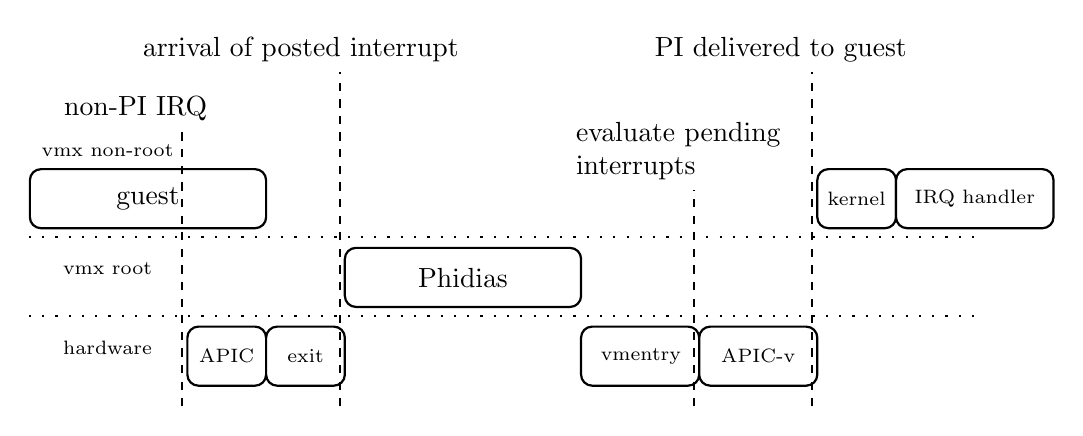
\begin{tikzpicture}

%\draw[step=1cm, gray, very thin, dotted] (0,0) grid (12,4);

\draw[black, thick, loosely dotted] (0,0.9) -- (12,0.9) node at (12,0.9) [below] {};
\draw[black, thick, loosely dotted] (0,1.9) -- (12,1.9) node at (12,1.9) [below] {};
\node at (1, 3) {\scriptsize{vmx non-root}};
\node at (1, 1.5) {\scriptsize{vmx root}};
\node at (1, 0.5) {\scriptsize{hardware}};


\node at (0,2) [rectangle, draw=black, thick, fill=white, rounded corners, minimum height = 0.75cm, minimum width = 3cm, anchor=south west] (gbefore) {guest};
\node at (2,0) [rectangle, draw=black, thick, fill=white, rounded corners, minimum height = 0.75cm, minimum width = 1cm, anchor=south west] (apic) {\scriptsize{APIC}};
\node at (3,0) [rectangle, draw=black, thick, fill=white, rounded corners, minimum height = 0.75cm, minimum width = 1cm, anchor=south west] (vmexit) {\scriptsize{exit}};
\node at (4,1) [rectangle, draw=black, thick, fill=white, rounded corners, minimum height = 0.75cm, minimum width = 3cm, anchor=south west] (phidias1) {Phidias};
\node at (7,0) [rectangle, draw=black, thick, fill=white, rounded corners, minimum height = 0.75cm, minimum width = 1.5cm, anchor=south west, text width=1cm] (entry) {\scriptsize{vmentry}};
\node at (8.5,0) [rectangle, draw=black, thick, fill=white, rounded corners, minimum height = 0.75cm, minimum width = 1.5cm, anchor=south west] (apicv) {\scriptsize{APIC-v}};

\draw[black, thick, dashed] (1.95,-0.25) -- (1.95, 3.25)  node [above, text width = 3cm] {non-PI IRQ};
\draw[black, thick, dashed] (3.95,-0.25) -- (3.95, 4.0)  node [above, text width = 5cm] {arrival of posted interrupt};
\draw[black, thick, dashed] (8.45,-0.25) -- (8.45, 2.5)  node [above, text width = 3cm] {evaluate pending interrupts};
\draw[black, thick, dashed] (9.95,-0.25) -- (9.95, 4.0)  node [above, text width = 4cm] {PI delivered to guest};

\node at (10,2) [rectangle, draw=black, thick, fill=white, rounded corners, minimum height = 0.75cm, minimum width = 1cm, anchor=south west] (gafter) {\scriptsize{kernel}};
\node at (11,2) [rectangle, draw=black, thick, fill=white, rounded corners, minimum height = 0.75cm, minimum width = 2cm, anchor=south west] (irqhandler) {\scriptsize{IRQ handler}};

\end{tikzpicture}
\end{center}
\caption{Posted interrupt worst case scenario}
\label{fig-pii-worstcase}
\end{figure}
